%%%%%%%%%%%%%%%%%%%%%%%%%%%%%%%%%%%%%%%%%%%%%%%%%%%%%%%%%%%%%%%%%%%%%%
% LaTeX Template: Curriculum Vitae
%
% Source: http://www.howtotex.com/
% Feel free to distribute this template, but please keep the
% referal to HowToTeX.com.
% Date: July 2011
% 
%%%%%%%%%%%%%%%%%%%%%%%%%%%%%%%%%%%%%%%%%%%%%%%%%%%%%%%%%%%%%%%%%%%%%%
% How to use writeLaTeX: 
%
% You edit the source code here on the left, and the preview on the
% right shows you the result within a few seconds.
%
% Bookmark this page and share the URL with your co-authors. They can
% edit at the same time!
%
% You can upload figures, bibliographies, custom classes and
% styles using the files menu.
%
% If you're new to LaTeX, the wikibook is a great place to start:
% http://en.wikibooks.org/wiki/LaTeX
%
%%%%%%%%%%%%%%%%%%%%%%%%%%%%%%%%%%%%%%%%%%%%%%%%%%%%%%%%%%%%%%%%%%%%%%

\documentclass{article}

\usepackage[margin=3.5cm]{geometry}
%\textheight=700px                    % Saving trees ;-)

%\setlength\parindent{0pt}
%\usepackage{parskip}
% Wrap long urls with hyphens
\PassOptionsToPackage{hyphens}{url}\usepackage{hyperref} 
% Underscores in doi break, the next command fixes that
\newcommand{\doi}[1]{\textsc{doi}: \href{http://dx.doi.org/#1}{\nolinkurl{#1}}}
\usepackage{comment}
\usepackage{ifplatform}
% Adding natbib adds \citet and \citep command
\usepackage[style=authoryear, natbib]{biblatex}
\usepackage{graphicx}
\usepackage{float}
% Pretty tables
\usepackage[table,xcdraw, svgnames]{xcolor}      % Colors by their 'svgnames'
\usepackage{tabularx}
\newcolumntype{b}{X}
\newcolumntype{s}{>{\hsize=.5\hsize}X}

\usepackage[english]{babel}
\usepackage[utf8]{inputenc}
\usepackage{csquotes}
\usepackage[protrusion=true,expansion=true]{microtype}
\usepackage{amsmath,amsfonts,amsthm}     % Math packages
\usepackage{graphicx}                    % Enable pdflatex
\usepackage{url}

\frenchspacing              % Better looking spacings after periods
\pagestyle{empty}           % No pagenumbers/headers/footers

%%% Custom sectioning (sectsty package)
%%% ------------------------------------------------------------
\usepackage{sectsty}

\sectionfont{%			            % Change font of \section command
	\usefont{OT1}{phv}{b}{n}%		% bch-b-n: CharterBT-Bold font
	\sectionrule{0pt}{0pt}{-5pt}{3pt}}

%%% Macros
%%% ------------------------------------------------------------
\newlength{\spacebox}
\settowidth{\spacebox}{8888888888}			% Box to align text
\newcommand{\sepspace}{\vspace*{1em}}		% Vertical space macro

\newcommand{\MyName}[1]{ % Name
		\Huge \usefont{OT1}{phv}{b}{n} \hfill #1
		\par \normalsize \normalfont}
		
\newcommand{\MySlogan}[1]{ % Slogan (optional)
		\large \usefont{OT1}{phv}{m}{n}\hfill \textit{#1}
		\par \normalsize \normalfont}

\newcommand{\NewPart}[1]{\section*{{\LARGE \color{Red}\#} \uppercase{#1}}}

\newcommand{\PersonalEntry}[2]{
		\noindent\hangindent=2em\hangafter=0 % Indentation
		\parbox{\spacebox}{        % Box to align text
		\textit{#1}}		       % Entry name (birth, address, etc.)
		\hspace{1.5em} #2 \par}    % Entry value

\newcommand{\SkillsEntry}[2]{      % Same as \PersonalEntry
		\noindent\hangindent=2em\hangafter=0 % Indentation
		\parbox{\spacebox}{        % Box to align text
		\textit{#1}}			   % Entry name (birth, address, etc.)
		\hspace{1.5em} #2 \par}    % Entry value	
		
\newcommand{\EducationEntry}[4]{
		\noindent \textbf{#1} \hfill      % Study
        \fbox{#2} \par
		%\colorbox{Black}{%
			%\parbox{6em}{%
			%\hfill\color{White}#2}} \par  % Duration
		\noindent \textit{#3} \par        % School
		\noindent\hangindent=2em\hangafter=0 \small #4 % Description
		\normalsize \par}

\newcommand{\WorkEntry}[4]{				  % Same as \EducationEntry
		\noindent \textbf{#1} \hfill      % Jobname
        \fbox{#2} \par
		%\colorbox{Black}{\color{White}#2} \par  % Duration
		\noindent \textit{#3} \par              % Company
		\noindent\hangindent=2em\hangafter=0 \small #4 % Description
		\normalsize \par}


%%% Extra customization
%%% ------------------------------------------------------------
\renewcommand{\thesubsection}{\number\numexpr\value{subsection}.\relax} %Do not show section number
\usepackage{wrapfig}

%%% Begin Document
%%% ------------------------------------------------------------
\begin{document}
% you can upload a photo and include it here...
\begin{wrapfigure}{r}{0.2\textwidth}
	\vspace*{-5em}
	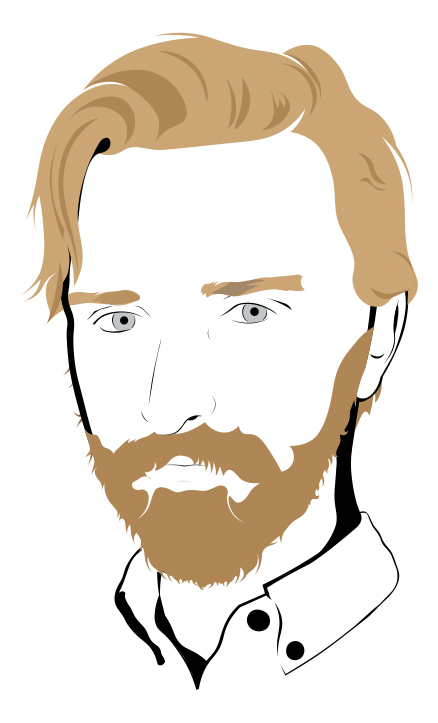
\includegraphics[width=0.15\textwidth]{img/ejw.jpg}
\end{wrapfigure}

% SET STRETCH
\baselinestretch

\MyName{Edwin Wenink}
%\MySlogan{Indian Institute of Engineering Science and Technology,Shibpur}
\MySlogan{Curriculum Vitae}

\sepspace

%%% Personal details
%%% ------------------------------------------------------------
\NewPart{Personal details}{}

\PersonalEntry{Name}{E.J. Wenink}
\PersonalEntry{Birth}{October 3, 1993}
\PersonalEntry{Mail}{\url{edwinwenink@hotmail.com}}
\PersonalEntry{Github}{\url{https://github.com/EdwinWenink}}
\PersonalEntry{LinkedIn}{\url{https://www.linkedin.com/in/ejwenink/}}
\PersonalEntry{Website}{\url{https://www.edwinwenink.xyz}}


%%% Education
%%% ------------------------------------------------------------
\NewPart{Education}{}

\EducationEntry{Master Artificial Intelligence}{2019-2022}{Radboud University}{Specialisation: Intelligent Technology\\
Thesis title: \emph{On the explainability of case law recommendations using paragraph embeddings}\\
Supervisors: Prof. dr. Tom van Engers and dr. Johan Kwisthout\\
GPA: 8.7\footnote{On a scale from 1 to 10.}, \emph{Cum laude}}

\sepspace

\EducationEntry{Research Master Philosophy}{2014-2020}{Radboud University}{Specialisation: Metaphysics and Epistemology\\
Thesis title: \emph{Destiny and adestination: Derrida and Heidegger on the sending of being}\\
Supervisor: Prof. dr. Gert-Jan van der Heiden\\
GPA: 8.3, \emph{Bene meritum}}

\sepspace

\EducationEntry{Bachelor Artificial Intelligence}{2016-2019}{Radboud University}{Thesis title: \textit{Query by Navigation over Legal Documents:\\
An Automated Pipeline using Formal Concept Analysis} \\
Supervisor: dr. Franc Grootjen, in cooperation with Wolters Kluwer \\
GPA: 8.7, \emph{Cum laude}}

\sepspace

\EducationEntry{Bachelor Philosophy}{2011-2014}{Radboud University}{Thesis title: \textit{Van Stem naar Arche-Schrift: Deconstructie in} De la Grammatologie\\
Supervisor: Prof. dr. Philippe van Haute
GPA: 8.8, \emph{Cum laude}}

\sepspace

\EducationEntry{Gymnasium}{2005-2011}{Thomas a Kempis college, Arnhem}{Graduated in two curricula: Nature and Technology, Nature and Health.\\ GPA: 8.5
}

%%% Honours, prizes, scholarships, grants
%%% ------------------------------------------------------------
\NewPart{Honours}{}

\EducationEntry{Honours Programme Philosophy, Theology\\ and Religious Studies}{2012-2014}{Radboud University}{On Schopenhauer's pessimistic metaphysics\\ Supervisor: Prof. dr. Ger Groot
}

\sepspace

%%% Work experience
%%% ------------------------------------------------------------
\NewPart{EXPERIENCE}{}

%%% ------------------------------------------------------------
\subsection*{1. Teaching and Tutoring}

\WorkEntry{Teaching Assistant Ethics for AI}{Mar.2021-Jul.2021}{Radboud University Nijmegen}{Chair working groups in the AI master\\ and contribute exam questions}
\sepspace

\WorkEntry{Teaching Assistant Societal Impact of AI}{Sep.2019-Feb.2020}{Radboud University Nijmegen}{Responsibilities: Teach working groups\\ and grade assignments and exams }
\sepspace

\WorkEntry{Teaching Assistant Introduction Artificial Intelligence}{Sep.2019-Nov.2019}{Radboud University Nijmegen}{Responsibilities: Teach working groups }
\sepspace

\WorkEntry{Teaching Assistant Theoretical Cognitive Science}{Feb.2019-Sep.2019}{Radboud University Nijmegen}{Responsibilities: Teach working groups\\ and grade assignments and exams }
\sepspace

\WorkEntry{Freelance Tutor for Student Recruitment Philosophy}{2014-2017}{Radboud University Nijmegen}{Chair working groups on university taster days}
\sepspace

\WorkEntry{Tutor in logic for philosophy students}{2011-2013}{}
\sepspace

\WorkEntry{Tutor in mathematics for high school students}{2009-2013}{}

%%% ------------------------------------------------------------
\subsection*{2. Internships}

\WorkEntry{Graduate Research Intern Explainable AI}{Sep.2021-Apr.2022}{TNO: Netherlands Organisation for Applied Scientific Research}{I worked on explainable recommendation of case law using text mining, embeddings, and counterfactual explanations. The internship took place within FATE, a flagship project of TNO's \href{https://appl-ai-tno.nl/}{\emph{Appl.ai}} program. FATE stands for FAir, Transparent and Explainable decision making.}

\sepspace

\WorkEntry{Intern Innovation Platform}{Mar.2021-Aug.2021}{NS: Netherlands Railways}{I helped realize an ethical approach to AI at NS by 1) working on AI policy and making it applicable to developers (ethics by design) and 2) researching tools and techniques for implementing values such as explainability and fairness.}

%%% ------------------------------------------------------------
\subsection*{3. Academic appointments}

\WorkEntry{Student Evaluation for the NVAO\\ Accreditation of Artificial Intelligence}{Nov.2018-Jan.2019}{Radboud University Nijmegen}{I was invited to participate in the self-evaluation\\of the study programme Artificial Intelligence\\ as needed for the accreditation by NVAO (every six years)}
\sepspace

\WorkEntry{Member of the Education Committee\\ Research Master Philosophy}{2015-2016}{Radboud University Nijmegen}{Main tasks: Reviewing the curriculum and providing recommendations\\ in cooperation with other advisory organs and the faculty board,\\ organizing social activities}
\sepspace

\WorkEntry{Member Nomination Committee for Assistant\\ Professor of the History of Philosophy}{Mar.2016}{Radboud University Nijmegen}{I was the student member of the nomination committee\\ that reviewed the candidate for the position of\\ Assistant Professor of the History of Philosophy}
\sepspace

\WorkEntry{Chairman on the Annual Deleuze Scholarship Conference}{Jun.2015}{Edition 4: Deleuze \& Aesthetics}{I chaired the parallel session ``Decentering subject matter'' }
\sepspace

%%% ------------------------------------------------------------
\NewPart{Papers and talks}

% TODO at some point introduce separate section and styling for paper references. This is quite informal now.
\WorkEntry{``Towards FAIR Explainable AI: a standardized ontology for mapping\\
XAI solutions to use cases, explanations, and AI systems.''}{2022}{A. Adhikari, \textbf{E. Wenink}, et al., \href{http://www.petrae.org/index.html}{PETRA 2022} (forthcoming).}
\sepspace

\WorkEntry{``E-Salon: social media, zegen of vloek voor het vrije debat?''}{2021}{Invited speaker by Stichting Vrij Links.\\
Event page: \url{https://www.vrij-links.nl/e-salon/social-media-zegen-of-vloek-voor-het-vrije-debat/}}
\sepspace

\WorkEntry{``Tech Giants will battle over your health data''}{2020}{Published in \textit{Turning Magazine}, Vol 2: AI \& Health, pp. 12-13.}
\sepspace

\WorkEntry{``Kunstmatige Intelligentie en haar gevolgen''}{2020}{Invited guest on the podcast \href{https://vocast.live/aflevering/kunstmatige-intelligentie/}{Vocast}}
\sepspace

\WorkEntry{Talk on ``Metaphysics and Metaphor in Heidegger's works''}{2016}{Joint Symposium of F.C. Sophia and Student Recruitment}
\sepspace

%TODO later vervangen door propere referenties
\WorkEntry{Undergraduate paper ``Deconstructie in werking''}{2013}{Published in \textit{Splijtstof} 42(2), pp. 49-58.}
\sepspace

\WorkEntry{Lecture (90 min.) on Schopenhauer's metaphysics\\
in \textit{Die Welt als Wille und Vorstellung}}{2012}{Graduation component of my honours programme}

%%% project
%%% ------------------------------------------------------------
\NewPart{Projects}{}

\WorkEntry{The AI Ethics Tool Landscape}{2021}{Editor, developer}{An open-source project that builds a taxonomy of practical tools for\\
implementing ethical AI.\\
Hosted at \url{https://edwinwenink.github.io/ai-ethics-tool-landscape/}}
\sepspace

\WorkEntry{Archive Fever: Website on Philosophy, Technology and AI}{2018-Present}{Editor, developer and writer}{Published 50+ online articles ranging from\\
	technical tutorials to philosophical essays.\\
	Currently 44.239 page views and 742 monthly unique visitors\\
	Hosted at \url{https://www.edwinwenink.xyz}
}
\sepspace

\WorkEntry{Elecast: Navigating Podcasts}{2020}{Developer}{A podcast app that allows navigation from audio segments to the\\ corresponding location in an AI-generated transcript and \textit{vice versa}.\\
Progressive Web App implemented in React.\\
Prototype at \url{https://nml-podcast-transcription.now.sh/player}}
\sepspace

\WorkEntry{CLIDE: A Clean IDE within Eclipse}{Sep.18-Feb.19}{Product owner by proxy, developer}{Scrum development of an IDE for the Clean functional\\ 
programming language, as an extension to the Eclipse framework.\\
As a product owner by proxy, I established product requirements\\
and priorities together with the client. \\
For information on Clean, see \url{https://clean.cs.ru.nl/Clean}}
\sepspace


%%% Skills
%%% ------------------------------------------------------------
\NewPart{Skills}{}

\SkillsEntry{Languages}{Dutch (mother tongue)}
\SkillsEntry{}{English (fluent)}
\SkillsEntry{}{German (working knowledge)}
\sepspace

\SkillsEntry{Programming Languages}{\textsc{Python}, \textsc{Java}, \textsc{R}, \textsc{Bash}}
\sepspace

\SkillsEntry{Frameworks}{\textsc{PyTorch}, \textsc{TensorFlow}, \textsc{scikit-learn}, \textsc{numpy}, \textsc{pandas}, \textsc{NLTK}, \textsc{gensim}}
\sepspace

\SkillsEntry{Software}{\textsc{Unix}, \textsc{Vim}, \LaTeX}
\sepspace

%%% References, 
%%% -----------------------------------------------------------
%\NewPart{Extra Curricular Activities}{}
%Available upon request
%1. Member of Society of Information Technology, IIEST, Shibpur
%\\
%\sepspace
%2. Swimming

\vspace*{\fill}
\small Last updated on \today.

\end{document}
